\section{Laboratory work implementation}

\subsection{Tasks and Points}

\begin{quote}
\begin{description}

	 Respectarea UX - Manipularea eventurilor de input gresit de catre utilizator \\
	Realizarea functiilor:\\
	Adunare;\\
	Scadere;\\
	Inmultire;\\
	Impartire;\\
	Ridicarea la putere;\\
	InversareSemn(+/-);\\
	Radical;\\
	Operatii cu numere zecimale;\\

\end{description}
\end{quote}

\subsection{Analiza lucrarii de laborator}

Am realizarea un software cu Sursa Cod si Sursa Grafica separat, acest proces de separare a fost automatizat de IDE-ul utilizat. Pe parcursul lucrarii am realizat un Calculator care permite efectuarea calculelor de baza. Am realizat o interfata grafica prietenoasa pentru utilizatori, ce permite utilizarea imediata a acestuia fara a apela la sursa Manual.


\subsection{Imagini}
\begin{figure}[htb]
	\begin{center}
		\centering
		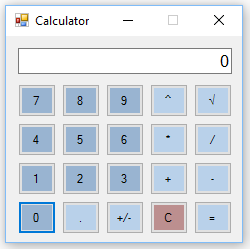
\includegraphics[scale = 1]{img/screenshot001.png}
		\caption{Interfata Calculatorului}%
		\label{fig:screenshot001}
	\end{center}
\end{figure}

\clearpage
